% ============================================================
% Kill-chain state machine with observation aliasing
% Compile with:  pdflatex state_machine_aliasing.tex
% Output:        state_machine_aliasing.pdf
% ============================================================
\documentclass[border=4pt]{standalone}
\usepackage{tikz}
\usetikzlibrary{shapes.geometric, arrows.meta, positioning, fit, backgrounds, calc}

\definecolor{colStage}{RGB}{220,235,245}
\definecolor{colBorder}{RGB}{80,100,120}
\definecolor{colArrow}{RGB}{60,80,100}
\definecolor{colAlias}{RGB}{180,140,120}

\tikzset{
  stateBox/.style={
    rectangle, rounded corners=3pt,
    draw=colBorder, line width=0.7pt,
    fill=colStage,
    text centered, font=\small,
    inner sep=5pt, minimum width=2.0cm, minimum height=1.4cm,
    align=center
  },
  arr/.style={
    -{Stealth[length=5pt]}, line width=0.8pt, color=colArrow
  },
  dasharr/.style={
    -{Stealth[length=5pt]}, line width=0.7pt, color=colAlias, dashed
  },
  label/.style={
    font=\footnotesize, text=colBorder
  }
}

\begin{document}
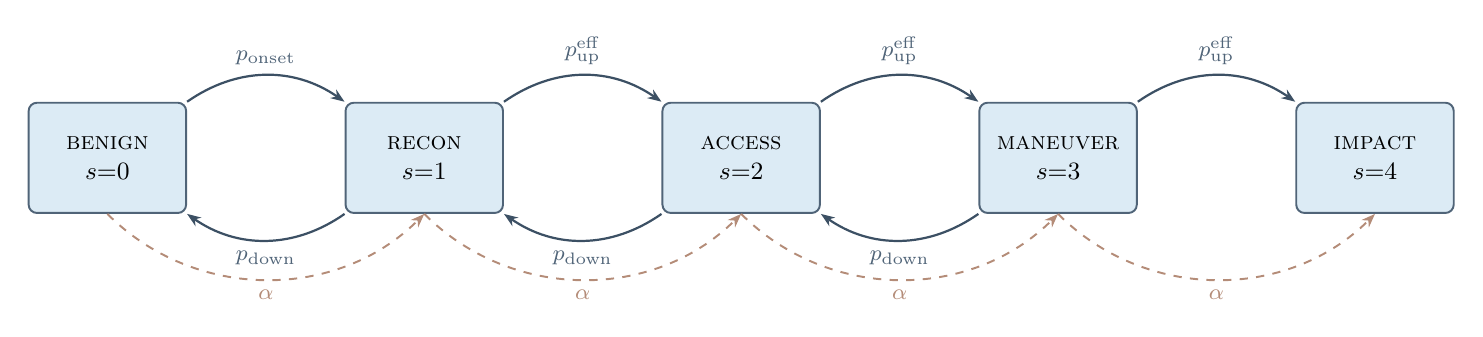
\begin{tikzpicture}[node distance=2.0cm]

  \node[stateBox] (s0) {\textsc{benign}\\$s{=}0$};
  \node[stateBox, right=of s0] (s1) {\textsc{recon}\\$s{=}1$};
  \node[stateBox, right=of s1] (s2) {\textsc{access}\\$s{=}2$};
  \node[stateBox, right=of s2] (s3) {\textsc{maneuver}\\$s{=}3$};
  \node[stateBox, right=of s3] (s4) {\textsc{impact}\\$s{=}4$};

  % escalation transitions (solid, above)
  \draw[arr] (s0.north east) to[bend left=35] node[label, above] {$p_{\mathrm{onset}}$} (s1.north west);
  \draw[arr] (s1.north east) to[bend left=35] node[label, above] {$p_{\mathrm{up}}^{\mathrm{eff}}$} (s2.north west);
  \draw[arr] (s2.north east) to[bend left=35] node[label, above] {$p_{\mathrm{up}}^{\mathrm{eff}}$} (s3.north west);
  \draw[arr] (s3.north east) to[bend left=35] node[label, above] {$p_{\mathrm{up}}^{\mathrm{eff}}$} (s4.north west);

  % de-escalation transitions (solid, below)
  \draw[arr] (s1.south west) to[bend left=35] node[label, below] {$p_{\mathrm{down}}$} (s0.south east);
  \draw[arr] (s2.south west) to[bend left=35] node[label, below] {$p_{\mathrm{down}}$} (s1.south east);
  \draw[arr] (s3.south west) to[bend left=35] node[label, below] {$p_{\mathrm{down}}$} (s2.south east);

  % observation aliasing (dashed, lower)
  \draw[dasharr] (s0.south) to[bend right=45] node[label, below, text=colAlias] {$\alpha$} (s1.south);
  \draw[dasharr] (s1.south) to[bend right=45] node[label, below, text=colAlias] {$\alpha$} (s2.south);
  \draw[dasharr] (s2.south) to[bend right=45] node[label, below, text=colAlias] {$\alpha$} (s3.south);
  \draw[dasharr] (s3.south) to[bend right=45] node[label, below, text=colAlias] {$\alpha$} (s4.south);

\end{tikzpicture}
\end{document}
